\documentclass[]{article}
\usepackage{lmodern}
\usepackage{amssymb,amsmath}
\usepackage{ifxetex,ifluatex}
\usepackage{fixltx2e} % provides \textsubscript
\ifnum 0\ifxetex 1\fi\ifluatex 1\fi=0 % if pdftex
  \usepackage[T1]{fontenc}
  \usepackage[utf8]{inputenc}
\else % if luatex or xelatex
  \ifxetex
    \usepackage{mathspec}
  \else
    \usepackage{fontspec}
  \fi
  \defaultfontfeatures{Ligatures=TeX,Scale=MatchLowercase}
\fi
% use upquote if available, for straight quotes in verbatim environments
\IfFileExists{upquote.sty}{\usepackage{upquote}}{}
% use microtype if available
\IfFileExists{microtype.sty}{%
\usepackage{microtype}
\UseMicrotypeSet[protrusion]{basicmath} % disable protrusion for tt fonts
}{}
\usepackage[margin=1in]{geometry}
\usepackage{hyperref}
\hypersetup{unicode=true,
            pdftitle={Assignment 4},
            pdfauthor={Mary Silva},
            pdfborder={0 0 0},
            breaklinks=true}
\urlstyle{same}  % don't use monospace font for urls
\usepackage{color}
\usepackage{fancyvrb}
\newcommand{\VerbBar}{|}
\newcommand{\VERB}{\Verb[commandchars=\\\{\}]}
\DefineVerbatimEnvironment{Highlighting}{Verbatim}{commandchars=\\\{\}}
% Add ',fontsize=\small' for more characters per line
\usepackage{framed}
\definecolor{shadecolor}{RGB}{248,248,248}
\newenvironment{Shaded}{\begin{snugshade}}{\end{snugshade}}
\newcommand{\KeywordTok}[1]{\textcolor[rgb]{0.13,0.29,0.53}{\textbf{#1}}}
\newcommand{\DataTypeTok}[1]{\textcolor[rgb]{0.13,0.29,0.53}{#1}}
\newcommand{\DecValTok}[1]{\textcolor[rgb]{0.00,0.00,0.81}{#1}}
\newcommand{\BaseNTok}[1]{\textcolor[rgb]{0.00,0.00,0.81}{#1}}
\newcommand{\FloatTok}[1]{\textcolor[rgb]{0.00,0.00,0.81}{#1}}
\newcommand{\ConstantTok}[1]{\textcolor[rgb]{0.00,0.00,0.00}{#1}}
\newcommand{\CharTok}[1]{\textcolor[rgb]{0.31,0.60,0.02}{#1}}
\newcommand{\SpecialCharTok}[1]{\textcolor[rgb]{0.00,0.00,0.00}{#1}}
\newcommand{\StringTok}[1]{\textcolor[rgb]{0.31,0.60,0.02}{#1}}
\newcommand{\VerbatimStringTok}[1]{\textcolor[rgb]{0.31,0.60,0.02}{#1}}
\newcommand{\SpecialStringTok}[1]{\textcolor[rgb]{0.31,0.60,0.02}{#1}}
\newcommand{\ImportTok}[1]{#1}
\newcommand{\CommentTok}[1]{\textcolor[rgb]{0.56,0.35,0.01}{\textit{#1}}}
\newcommand{\DocumentationTok}[1]{\textcolor[rgb]{0.56,0.35,0.01}{\textbf{\textit{#1}}}}
\newcommand{\AnnotationTok}[1]{\textcolor[rgb]{0.56,0.35,0.01}{\textbf{\textit{#1}}}}
\newcommand{\CommentVarTok}[1]{\textcolor[rgb]{0.56,0.35,0.01}{\textbf{\textit{#1}}}}
\newcommand{\OtherTok}[1]{\textcolor[rgb]{0.56,0.35,0.01}{#1}}
\newcommand{\FunctionTok}[1]{\textcolor[rgb]{0.00,0.00,0.00}{#1}}
\newcommand{\VariableTok}[1]{\textcolor[rgb]{0.00,0.00,0.00}{#1}}
\newcommand{\ControlFlowTok}[1]{\textcolor[rgb]{0.13,0.29,0.53}{\textbf{#1}}}
\newcommand{\OperatorTok}[1]{\textcolor[rgb]{0.81,0.36,0.00}{\textbf{#1}}}
\newcommand{\BuiltInTok}[1]{#1}
\newcommand{\ExtensionTok}[1]{#1}
\newcommand{\PreprocessorTok}[1]{\textcolor[rgb]{0.56,0.35,0.01}{\textit{#1}}}
\newcommand{\AttributeTok}[1]{\textcolor[rgb]{0.77,0.63,0.00}{#1}}
\newcommand{\RegionMarkerTok}[1]{#1}
\newcommand{\InformationTok}[1]{\textcolor[rgb]{0.56,0.35,0.01}{\textbf{\textit{#1}}}}
\newcommand{\WarningTok}[1]{\textcolor[rgb]{0.56,0.35,0.01}{\textbf{\textit{#1}}}}
\newcommand{\AlertTok}[1]{\textcolor[rgb]{0.94,0.16,0.16}{#1}}
\newcommand{\ErrorTok}[1]{\textcolor[rgb]{0.64,0.00,0.00}{\textbf{#1}}}
\newcommand{\NormalTok}[1]{#1}
\usepackage{graphicx,grffile}
\makeatletter
\def\maxwidth{\ifdim\Gin@nat@width>\linewidth\linewidth\else\Gin@nat@width\fi}
\def\maxheight{\ifdim\Gin@nat@height>\textheight\textheight\else\Gin@nat@height\fi}
\makeatother
% Scale images if necessary, so that they will not overflow the page
% margins by default, and it is still possible to overwrite the defaults
% using explicit options in \includegraphics[width, height, ...]{}
\setkeys{Gin}{width=\maxwidth,height=\maxheight,keepaspectratio}
\IfFileExists{parskip.sty}{%
\usepackage{parskip}
}{% else
\setlength{\parindent}{0pt}
\setlength{\parskip}{6pt plus 2pt minus 1pt}
}
\setlength{\emergencystretch}{3em}  % prevent overfull lines
\providecommand{\tightlist}{%
  \setlength{\itemsep}{0pt}\setlength{\parskip}{0pt}}
\setcounter{secnumdepth}{0}
% Redefines (sub)paragraphs to behave more like sections
\ifx\paragraph\undefined\else
\let\oldparagraph\paragraph
\renewcommand{\paragraph}[1]{\oldparagraph{#1}\mbox{}}
\fi
\ifx\subparagraph\undefined\else
\let\oldsubparagraph\subparagraph
\renewcommand{\subparagraph}[1]{\oldsubparagraph{#1}\mbox{}}
\fi

%%% Use protect on footnotes to avoid problems with footnotes in titles
\let\rmarkdownfootnote\footnote%
\def\footnote{\protect\rmarkdownfootnote}

%%% Change title format to be more compact
\usepackage{titling}

% Create subtitle command for use in maketitle
\newcommand{\subtitle}[1]{
  \posttitle{
    \begin{center}\large#1\end{center}
    }
}

\setlength{\droptitle}{-2em}

  \title{Assignment 4}
    \pretitle{\vspace{\droptitle}\centering\huge}
  \posttitle{\par}
    \author{Mary Silva}
    \preauthor{\centering\large\emph}
  \postauthor{\par}
      \predate{\centering\large\emph}
  \postdate{\par}
    \date{3/13/2019}


\begin{document}
\maketitle

\subsection{1A}\label{a}

Using \(\theta_1 = 1.5\) and \(\theta_2 = 2\) we draw a sample of size
1000 using the independence Metropolis Hastings algorithm with gamma
distribution as the proposal density.

\begin{Shaded}
\begin{Highlighting}[]
\NormalTok{theta_}\DecValTok{1}\NormalTok{ =}\StringTok{ }\FloatTok{1.5} \CommentTok{# true value theta1}
\NormalTok{theta_}\DecValTok{2}\NormalTok{ =}\StringTok{ }\DecValTok{2} \CommentTok{# true value theta2}
\NormalTok{mean_z1 =}\StringTok{ }\KeywordTok{sqrt}\NormalTok{(theta_}\DecValTok{2}\OperatorTok{/}\NormalTok{theta_}\DecValTok{1}\NormalTok{)}
\NormalTok{mean_z2 =}\StringTok{ }\KeywordTok{sqrt}\NormalTok{(theta_}\DecValTok{1}\OperatorTok{/}\NormalTok{theta_}\DecValTok{2}\NormalTok{) }\OperatorTok{+}\StringTok{ }\DecValTok{1}\OperatorTok{/}\NormalTok{(}\DecValTok{2}\OperatorTok{*}\NormalTok{theta_}\DecValTok{2}\NormalTok{)}

\CommentTok{# hyperparams}
\NormalTok{b =}\StringTok{ }\FloatTok{2.5}
\NormalTok{a =}\StringTok{ }\NormalTok{mean_z1}\OperatorTok{*}\NormalTok{b}
\CommentTok{#M-H Algorithm}
\NormalTok{MH_alg1 =}\StringTok{ }\ControlFlowTok{function}\NormalTok{(N)\{}
\NormalTok{  MH_samples =}\StringTok{ }\KeywordTok{rep}\NormalTok{(}\OtherTok{NA}\NormalTok{, N)}
\NormalTok{  count =}\StringTok{ }\DecValTok{0}
\NormalTok{  current_z =}\StringTok{ }\FloatTok{1.0}
  \ControlFlowTok{for}\NormalTok{(i }\ControlFlowTok{in} \DecValTok{1}\OperatorTok{:}\NormalTok{N)\{}
\NormalTok{    curr_p =}\StringTok{ }\KeywordTok{pdf_z}\NormalTok{(current_z) }
\NormalTok{    z_new =}\StringTok{ }\KeywordTok{rgamma}\NormalTok{(}\DecValTok{1}\NormalTok{, a, b)}
\NormalTok{    p_new =}\StringTok{ }\KeywordTok{pdf_z}\NormalTok{(z_new)}
    
\NormalTok{    accept =}\StringTok{ }\KeywordTok{exp}\NormalTok{(p_new }\OperatorTok{+}\StringTok{ }\KeywordTok{dgamma}\NormalTok{(current_z,a,b,}\DataTypeTok{log =}\NormalTok{ T) }\OperatorTok{-}\StringTok{ }\NormalTok{p_new }\OperatorTok{-}\StringTok{ }\KeywordTok{dgamma}\NormalTok{(z_new,a,b,}\DataTypeTok{log =}\NormalTok{ T))}
    \ControlFlowTok{if}\NormalTok{(}\KeywordTok{runif}\NormalTok{(}\DecValTok{1}\NormalTok{) }\OperatorTok{<}\StringTok{ }\NormalTok{accept)\{}
\NormalTok{      current_z =}\StringTok{ }\NormalTok{z_new}
\NormalTok{      count =}\StringTok{ }\NormalTok{count }\OperatorTok{+}\StringTok{ }\DecValTok{1}
\NormalTok{    \}}
\NormalTok{    MH_samples[i] =}\StringTok{ }\NormalTok{current_z}
\NormalTok{  \}}
  \KeywordTok{return}\NormalTok{(}\KeywordTok{list}\NormalTok{(}\DataTypeTok{MH_samples=}\NormalTok{MH_samples,}\DataTypeTok{count=}\NormalTok{count))}
\NormalTok{\}}
\end{Highlighting}
\end{Shaded}

After trying several hyperparameters for different Gamma distributions,
the best sample obtains a mean, \(E(Z)\), of

\begin{verbatim}
## [1] 1.763996
\end{verbatim}

\(E(1/Z)\)

\begin{verbatim}
## [1] 1.537128
\end{verbatim}

and an accuracy of

\begin{verbatim}
## [1] 0.513
\end{verbatim}

The traceplot for the samples for Metropolis-Hastings is shown below:

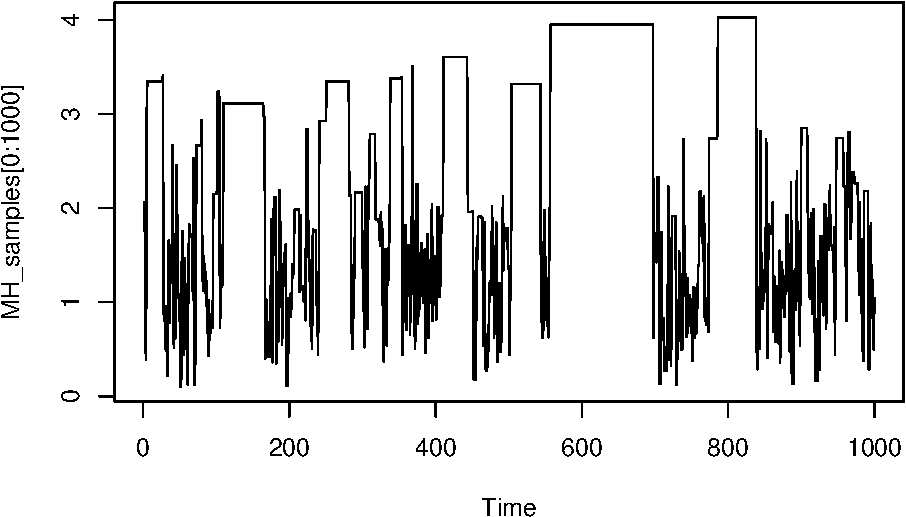
\includegraphics{AMS206b_H4_files/figure-latex/unnamed-chunk-5-1.pdf}

\subsection{1B}\label{b}

The density of \(W = log(Z)\) is given by
\[ f_W(w) \propto \exp\left\{- \frac{3}{2} w - \theta_1 exp\{w\} - \frac{\theta_2}{\exp(w)} \right\} \exp(w) \]

We draw a sample of size 1000 using the random-walk Metropolis algorithm
with this density.

\begin{Shaded}
\begin{Highlighting}[]
\NormalTok{v =}\StringTok{ }\FloatTok{0.01}
\NormalTok{MH_RW =}\StringTok{ }\ControlFlowTok{function}\NormalTok{(N)\{}
\NormalTok{  N =}\StringTok{ }\NormalTok{N}
\NormalTok{  MH_RW =}\StringTok{ }\KeywordTok{rep}\NormalTok{(}\OtherTok{NA}\NormalTok{, N)}
\NormalTok{  a_count =}\StringTok{ }\DecValTok{0}
\NormalTok{  z_curr =}\StringTok{ }\FloatTok{1.0}
  \ControlFlowTok{for}\NormalTok{ (i }\ControlFlowTok{in} \DecValTok{1}\OperatorTok{:}\NormalTok{N) \{}
\NormalTok{    p_curr =}\StringTok{ }\KeywordTok{pdf_z2}\NormalTok{(z_curr)}
\NormalTok{    z_new =}\StringTok{ }\KeywordTok{exp}\NormalTok{(}\KeywordTok{log}\NormalTok{(z_curr) }\OperatorTok{+}\StringTok{ }\KeywordTok{rnorm}\NormalTok{(}\DecValTok{1}\NormalTok{,}\DecValTok{0}\NormalTok{,}\KeywordTok{sqrt}\NormalTok{(v)))}
\NormalTok{    p_new =}\StringTok{ }\KeywordTok{pdf_z2}\NormalTok{(z_new)}
\NormalTok{    acceptance =}\StringTok{ }\KeywordTok{exp}\NormalTok{(p_new }\OperatorTok{-}\StringTok{ }\NormalTok{p_curr)}
    \ControlFlowTok{if}\NormalTok{(}\KeywordTok{runif}\NormalTok{(}\DecValTok{1}\NormalTok{) }\OperatorTok{<}\StringTok{ }\NormalTok{acceptance)\{}
\NormalTok{      z_curr =}\StringTok{ }\NormalTok{z_new}
\NormalTok{      a_count =}\StringTok{ }\NormalTok{a_count}\OperatorTok{+}\DecValTok{1}
\NormalTok{    \}}
\NormalTok{    MH_RW[i] =}\StringTok{ }\NormalTok{z_curr}
\NormalTok{  \}}
  \KeywordTok{return}\NormalTok{(}\KeywordTok{list}\NormalTok{(}\DataTypeTok{MH_RW=}\NormalTok{MH_RW, }\DataTypeTok{a_count=}\NormalTok{a_count))}
\NormalTok{\}}
\end{Highlighting}
\end{Shaded}

The mean for the samples is

\begin{verbatim}
## [1] 1.114488
\end{verbatim}

And the accuracy is

\begin{verbatim}
## [1] 0.9363
\end{verbatim}

If we use 10000 metropolis hastings random ralk samples, the traceplot
is shown below

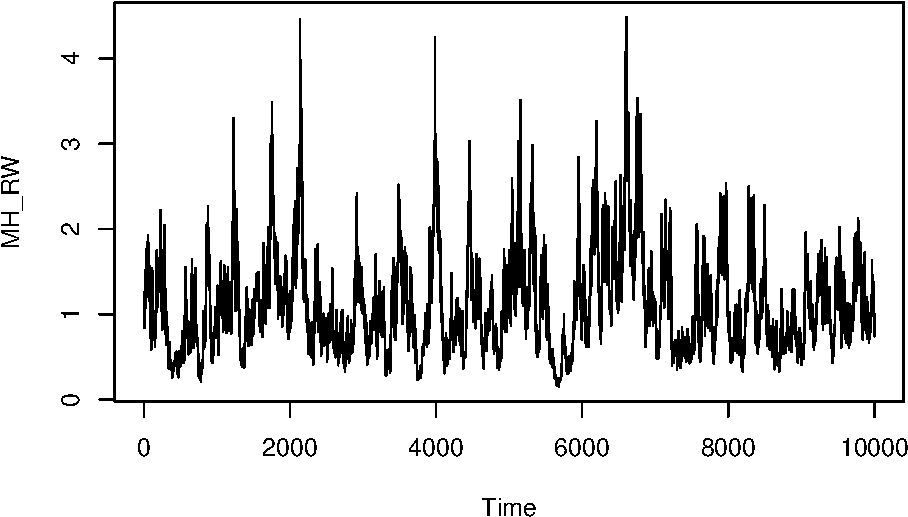
\includegraphics{AMS206b_H4_files/figure-latex/unnamed-chunk-11-1.pdf}

\subsection{2A}\label{a-1}

\[x_i |\nu,\theta \sim Gamma(\nu,\theta)\] \[\nu \sim Gamma(a,b)\]
\[\theta \sim Gamma(\alpha,\beta)\] The joint posterior for \(\theta\)
and \(\nu\)
\[\pi(\theta,\nu,\pmb{x}) \propto  \frac{\left(\prod_{i=1}^nx_i \right)^{\nu-1}\nu^{a-1} e^{-b\nu}}{\left(\Gamma(\nu) \right)^n} \theta^{a+n\nu-1} \exp\left\{-\theta\left(\beta + \sum_{i=1}^n x_i \right) \right\}\]

The full conditionals:
\[\pi(\theta|\nu, \pmb{x}) \propto \theta^{a+n\nu-1}\exp\left\{-\theta\left(\beta + \sum_{i=1}^n x_i \right) \right\}\]

thus, \(\theta|\nu, \pmb{x} \sim Gamma(n\nu, \beta + \sum x_i)\).

\[\pi(\nu|\theta,\pmb{x}) \propto \theta^{n\nu}\frac{\left(\prod_{i=1}^nx_i \right)^{\nu-1}\nu^{a-1} e^{-b\nu}}{\left(\Gamma(\nu) \right)^n}\]


\end{document}
